\title{As ``outras'' revistas científicas}
\author{por Vidal Barrón}
\maketitle
\begin{wrapfigure}{l}{0.15\textwidth}
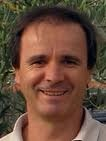
\includegraphics[width=0.15\textwidth]{figuras/foto-vidal-barron}
\end{wrapfigure}

Em 1887 a revista \href{http://www.ajsonline.org/}{\textit{American Journal of Science}}, a mais antiga dos Estados Unidos, publicou um artigo intitulado ``\textit{On the Relative Motion of the Earth and the Luminiferous Ether}''. Nesse trabalho, não foi encontrada nenhuma relação entre o movimento relativo da Terra e o suposto ``éter luminoso''. O mesmo autor desse trabalho, Albert A. Michelson, recebeu em 1907 o Prêmio Nobel de Física, pelo desenvolvimento do interferômetro, aparelho utilizado para efetuar medidas de ângulos e distâncias aproveitando a interferência de ondas electromagnéticas.

Provavelmente muitas de nossas experiências fracassadas ou negativas nunca chegaram à relevância do trabalho de Michelson. No entanto, em muitos campos da ciência a publicação de resultados inesperados podem ser de grande importância, não só porque evita que erros sejam cometidos novamente resultando em desperdício econômico, mas em alguns casos, porque ajuda a negar ideias ou hipóteses, e a criar novas.

A meta-análise, estudos que utilizam técnicas estatísticas para combinar resultados independentes sobre investigação em áreas como medicina, farmácia, biologia ou agronomia são tendenciosos. A pressão por parte das agencias financiadoras, e até mesmo a autocensura, leva muitos pesquisadores a não publicarem resultados negativos ou melhor, publicarem em revistas de baixo impacto. 

A fim de superar essas falhas da ``máquina científica'', nasceram várias revistas que coletam estes resultados inesperados, frustrantes ou negativos. Abrangendo diversas áreas do conhecimento científico, como química, física, biologia ou nanotecnologia, desde 2010 existe a \href{http://www.arjournals.com/ojs/}{\textit{The All Results Journals}}, uma revista de acesso aberto, ou seja, nem os leitores nem os autores têm que pagar para ler e/ou publicar seus artigos. Outras revistas como \href{http://www.jnrbm.com/}{\textit{Journal of Negative Results in BioMedicine}} e \href{http://www.pnrjournal.com/}{\textit{Journal of Pharmaceutical Negative Results}} também seguem essa filosofia de publicação de resultados inesperados. Muitas outras áreas, por exemplo, agronomia também poderiam se beneficiar de uma plataforma para a publicação e discussão de resultados inesperados, polêmicos, provocativos e/ou negativos.

E se os nossos resultados, embora gerados com o rigor científico necessário, também tivessem um toque de humor inesperado ou previsto? \href{http://www.jir.com/index.html}{\textit{The Journal of Irreproducible Results}} oferece a possibilidade de publicar todos os tipos de piadas, paródias, sátira e humor gráfico de caráter científico. Com mentalidade parecida, porém com maior índice de impacto, existe a \href{http://www.improbable.com/}{\textit{Annals of Improbable Research}}, editada pela prestigiada Universidade de Harvard. Esta revista  também é conhecida pelo famoso Prêmio \href{http://www.improbable.com/ig/winners/}{\textit{IgNobel}}, dado para a descoberta científica mais estranha do ano em diferentes campos da ciência. Alguns ganhadores do \textit{IgNobel} foram: Len Fisher em 1999, por sua pesquisa sobre a física de como molhar um biscoito. Lendo sua pesquisa, agora convertido em um livro \textit{best-seller}, nos inspirou no passado, a interpretar o comportamento de alguns solos brasileiros. Outro conhecido ganhador do \textit{IgNobel} foi o pesquisador Andre Geim, ganhador do Prêmio Nobel de Física em 2010 por suas pesquisas sobre o grafeno. Geim, recebeu em 2000 o \textit{IgNobel} pelo seu estudo sobre a levitação de rãs em um campo magnético. Parece, que este tipo de publicação pode ser o prelúdio de conquistas cientificas maiores!

\address{Vidal Barrón\\
  Universidade de Córdoba, UCO, Espanha\\
  \url{http://www.researchgate.net/profile/Vidal\_Barron}\\
  \email{cr1balov@uco.es}}
%%% Local Variables: 
%%% mode: latex
%%% TeX-master: 4th-edition.tex
%%% End: 